%!TEX TS-program = xelatex
%!TEX encoding = UTF-8 Unicode

\documentclass[12pt]{article}
\usepackage{geometry}                % See geometry.pdf to learn the layout options. There are lots.
\geometry{a4paper,top=2cm}
\usepackage[parfill]{parskip}    % Activate to begin paragraphs with an empty line rather than an indent
\usepackage{graphicx}
\usepackage{amsmath}
\usepackage{amssymb}
\usepackage{mathtools}
\usepackage{physics}
\newcommand{\be}{\begin{equation}}
\newcommand{\ee}{\end{equation}}
\usepackage[thicklines]{cancel}
\usepackage[colorlinks=true,citecolor=blue,linkcolor=blue,urlcolor=blue]{hyperref}
\usepackage{booktabs}
\usepackage{csquotes}
\usepackage{qcircuit}
\usepackage{circledsteps}
\usepackage{nicefrac}
\usepackage{fontspec,xltxtra,xunicode}
\usepackage{xcolor}
\usepackage{simplewick}
\defaultfontfeatures{Mapping=tex-text}

\newcommand{\polv}{\ensuremath{\updownarrow}}
\newcommand{\polh}{\ensuremath{\leftrightarrow}}
\newcommand{\poldr}{\rotatebox[origin=c]{45}{\ensuremath{\leftrightarrow}}}
\newcommand{\poldl}{\rotatebox[origin=c]{-45}{\ensuremath{\leftrightarrow}}}
\newcommand{\bigzero}{\mbox{\normalfont\Large\bfseries 0}}
\newcommand{\vecrp}{\ensuremath{\vec{r}^{\,\prime}}}
\newcommand{\vecnr}{\ensuremath{\vec{\nabla}_{\!r}}}

\title{Advanced Quantum Mechanics\\Class 18 (a)}
%\author{The Author}
\date{April 20, 2023}                                           % Activate to display a given date or no date

\setcounter{section}{4}
\setcounter{subsection}{5}
\setcounter{equation}{44}

\begin{document}
\maketitle

%%% 01 OKAY
\subsection{Lie algebra associated with rotation group}

Let us consider the rotation of a vector $\vec{V}$ by an angle $\theta$
about an arbitrary axis $\hat{n}$\\%Force this linebreak
\be
g \to R_{\hat{n}}(\theta) = e^{-i\theta(\hat{n}\cdot\hat{\vec{T}})}
\label{eq:g45}
\ee
where $R$ is a $3\times3$ matrix, so $\vec{T}$ is a vector $(T_1, T_2, T_3)$ of $3\times3$ matrices.

\begin{minipage}{0.5\textwidth}
\hspace{8ex}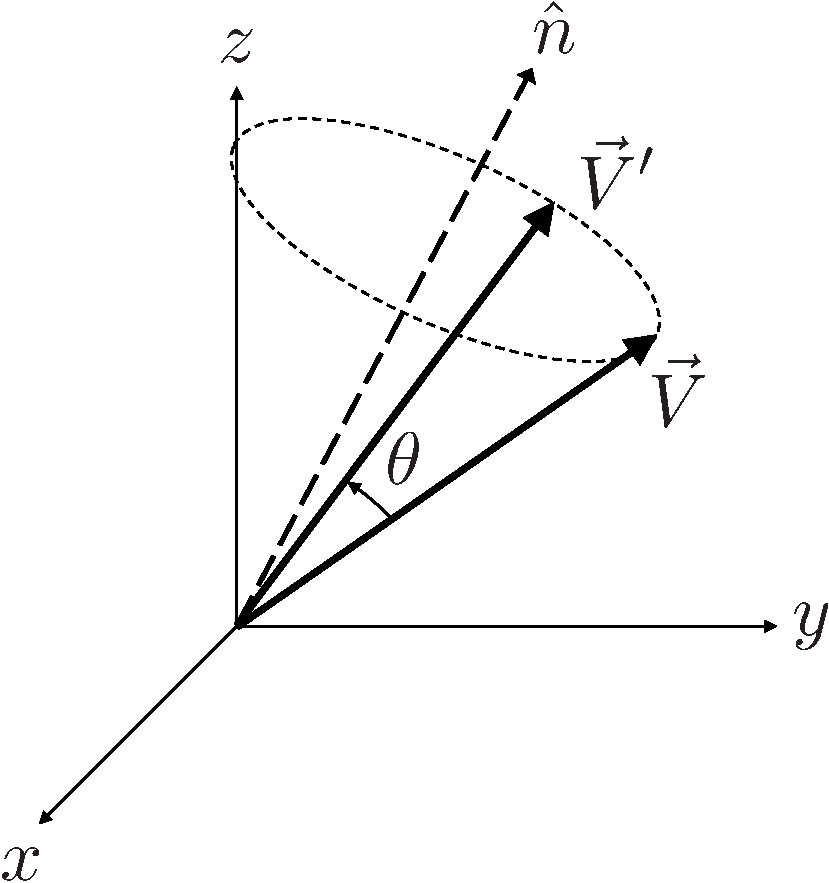
\includegraphics[width=0.6\textwidth]{Figures/detailedRotation-crop.pdf}
\end{minipage}%
\begin{minipage}{0.5\textwidth}
\begin{tabular}{ll}
$\|$ :    & parallel to $\hat{n}$\\
$\perp$ : & perpendicular to $\hat{n}$\\[0.5ex]
\end{tabular}\\
\be
\left.
\begin{aligned}
\vec{V} = \vec{V_\|} + \vec{V_\perp}\\
\vec{V}^{\prime} = \vec{V_\|}^\prime + \vec{V_\perp}^\prime
\end{aligned}
\right\}
\|\vec{V}^{\prime}\| = \|\vec{V}\|
\ee
\be
\begin{aligned}
\vec{V_\|} &= (\hat{n} \cdot \vec{V})\,\hat{n}\\
\vec{V_\perp} &= \vec{V} - (\hat{n} \cdot \vec{V})\,\hat{n}
\end{aligned}
\ee
\end{minipage}%

Rotation does not change the component parallel to $\hat{n}$:
\be
\vec{V_\|}^\prime = \vec{V}_{\|} = (\vec{V} \cdot \hat{n}) \hat{n}
\ee 

%%% 02 OKAY
Look then in the transverse direction to $\hat{n}$:
\setcounter{equation}{47}

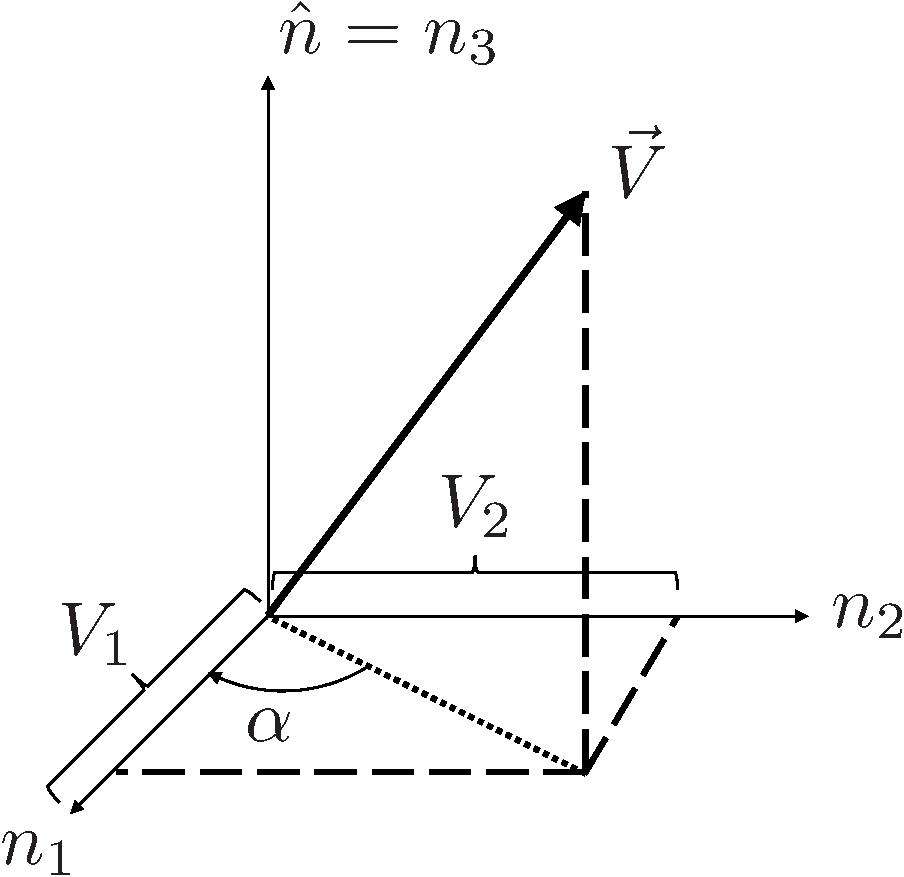
\includegraphics[width=0.4\textwidth]{Figures/transverseRotation-crop.pdf}
\raisebox{2cm}{\begin{tabular}{c}
in the\\
$(n_1,n_2)$ plane\\
$-\hspace{-0.5em}-\hspace{-0.5em}-\hspace{-0.5em}\longrightarrow$\\
\end{tabular}}
\raisebox{1.5em}{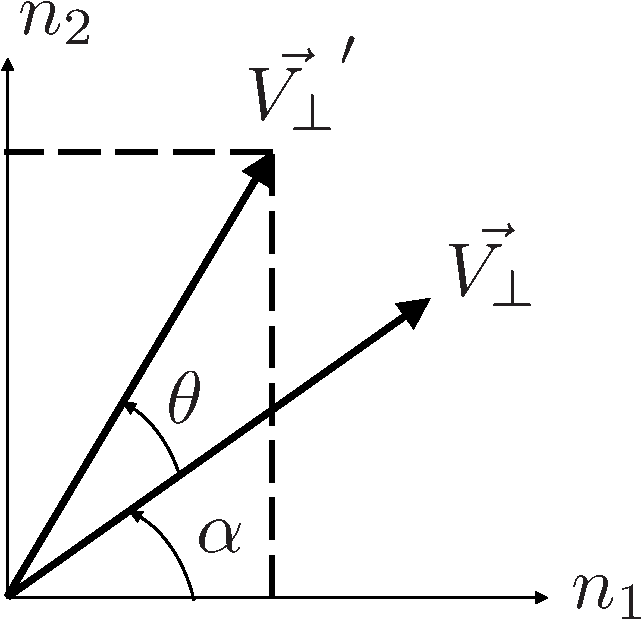
\includegraphics[width=0.3\textwidth]{Figures/transverseRotation2-crop.pdf}}

\be
\begin{aligned}
(\vec{V_\perp}^\prime)_1 
&= \vec{V_\perp}^\prime \cos(\alpha+\theta) = \underbrace{V_\perp^\prime \cos\alpha}%
_{(\vec{V_\perp})_1} \cos\theta -  \underbrace{V_\perp^\prime \sin\alpha}%
_{(\vec{V_\perp})_2}\sin\theta\\
&=(\vec{V_\perp})_1 \cos\theta - (\vec{V_\perp})_2 \sin\theta
\end{aligned}
\label{eq:g48}
\ee
%
\be
\begin{aligned}
(\vec{V_\perp}^\prime)_2 
&= \vec{V_\perp} \sin(\alpha+\theta) = \underbrace{V_\perp \sin\alpha}%
_{(\vec{V_\perp})_2} \cos\theta -  \underbrace{V_\perp \cos\alpha}%
_{(\vec{V_\perp})_1}\sin\theta\\
&=(\vec{V_\perp})_2 \cos\theta + (\vec{V_\perp})_1 \sin\theta
\end{aligned}
\label{eq:g49}
\ee
Eqs.~\eqref{eq:g48}--\eqref{eq:g49} can be summarized as
\be
\begin{aligned}
\vec{V_\perp}^\prime 
&= \vec{V_\perp} \cos\theta + (\hat{n} \times \vec{V}) \sin\theta\\
&=[\vec{V} - (\hat{n}\cdot\vec{V})\hat{n}] \cos\theta + (\hat{n} \times \vec{V}) \sin\theta
\end{aligned}
\ee
so
\be
\vec{V}^{\,\prime}  = (1-\cos\theta)(\hat{n}\cdot\vec{V})\hat{n} + \cos\theta\,\vec{V} + \sin\theta (\hat{n} \times \vec{V})
\label{eq:fullExpressionRotation}
\ee
For $\theta$ infinitesimal, $\theta \to 0$: Eqs.~\eqref{eq:g45} and \eqref{eq:fullExpressionRotation} lead to
\be
 R_{\hat{n}}(\theta) \simeq I -i\theta(\hat{n}\cdot\hat{\vec{T}})
\label{eq:g52}
\ee
\be
\vec{V}^{\,\prime} = \vec{V} + \theta(\vec{n} \times \vec{V})
\label{eq:g53}
\ee
%%% 03 OKAY
From Eqs.~\eqref{eq:g52} and \eqref{eq:g53}: (implicit sum over repeated indices)
\be
V_i^\prime = [\delta_{ij} - i\theta(\hat{n}\cdot \hat{T})_{ij}] V_j
		   = [\delta_{ij} +  \theta(\hat{n}\times\vec{V})_{ij}] V_j
\ee
whence
\be
-i(\hat{n}\cdot\overleftrightarrow{T})_{ij} V_j 
= (\hat{n}\times\vec{V})_i
= \epsilon_{ijk} \hat{n}_j V_k
\ee
which means
\be
\begin{aligned}
-i(\hat{n}\cdot\hat{\overleftrightarrow{T}})\vec{V} =
\begin{cases}
0 V_x -n_z V_y +n_y V_z\\
n_z V_x + 0 V_y -n_x V_z\\
-n_y V_x + n_x V_y + 0 V_z
\end{cases}\\[1ex]
=\begin{pmatrix}
0 & -n_z & n_y\\
n_z & 0 & -n_x\\
-n_y & n_x & 0\\
\end{pmatrix}
\begin{pmatrix}
V_x \\ V_y \\ V_z
\end{pmatrix}
\end{aligned}
\ee
Writing:
\be
(\hat{n}\cdot\hat{\overleftrightarrow{T}})_{ij} = 
(n_x \hat{T}_x + n_y \hat{T}_y + n_z \hat{T}_z)_{ij}
\ee
\be
T_x = \begin{pmatrix} 0 & 0 &  0\\ 0 & 0 & -i\\ 0 & i &  0\end{pmatrix},\quad
T_y = \begin{pmatrix} 0 & 0 &  i\\ 0 & 0 &  0\\-i & 0 &  0\end{pmatrix},\quad
T_z = \begin{pmatrix} 0 &-i &  0\\ i & 0 &  0\\ 0 & 0 &  0\end{pmatrix},\quad
\ee
which are the matrices that generate the rotation in \emph{real} space.
%%% 04 OKAY
By direct calculation, one can verify that these
matrices satisfy the following commutation relations:
\be
[T_i,T_j] = i\,\epsilon_{ijk}\,T_k
\label{eq:g59}
\ee
\rule{\textwidth}{1pt}
A more direct way to derive this:
\begin{enumerate}
\item Choose a frame in which $\hat{n}$ is contained in the $y O z$ plane.
Then you can decompose $R_{\hat{n}(\phi)}(\theta) = e^{-i\theta \hat{n}(\phi)\cdot T}$ in:\\[0.6em]
\begin{minipage}{0.35\textwidth}
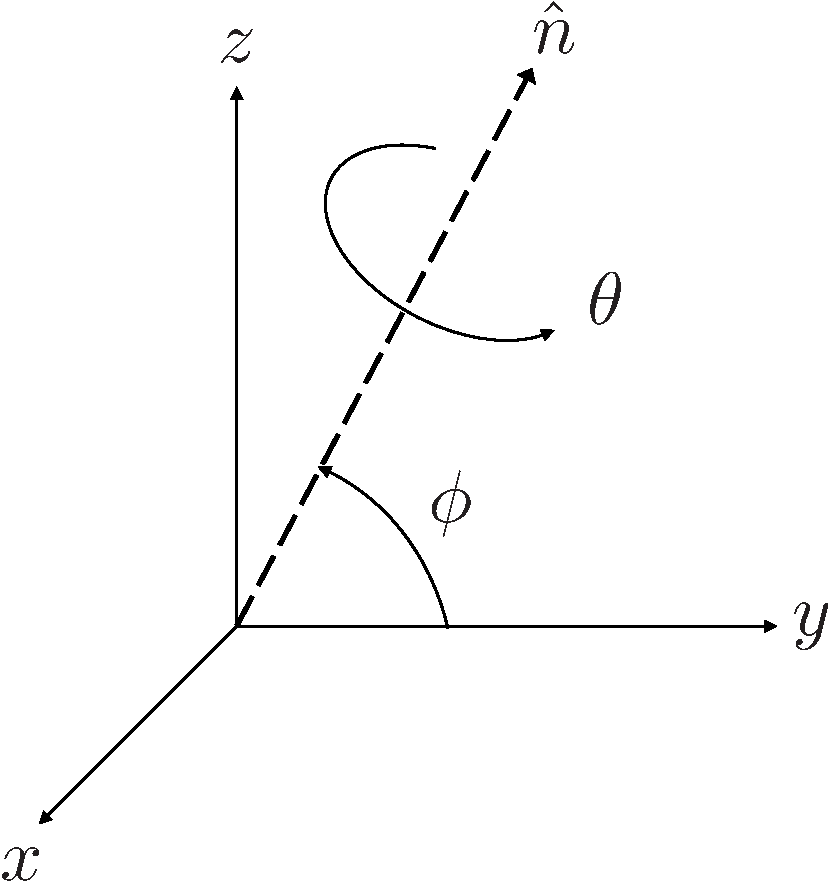
\includegraphics[width=\textwidth]{Figures/simpleRotation-crop.pdf}
\end{minipage}%
\begin{minipage}{0.65\textwidth}
\be
R_{\hat{n}(\phi)}(\theta) \equiv R_x(\phi)\, R_y(\theta)\, R_x(-\phi)	
\ee
\end{minipage}\\[0.6em]%
where 
$R_x(-\phi)  = e^{ i\phi T_x}$ brings $\hat{n}$ to the $Oy$ axis,
$R_y(\theta) = e^{-i\theta T_y}$ gets the aimed rotation, and
$R_x( \phi)  = e^{-i\phi T_x}$ puts $\hat{n}$ back to its original direction. 
Now, for $\theta \to 0$:
\[
\begin{gathered}
(1 - i\theta \hat{n}(\phi)\cdot T) = e^{-i\phi T_x} (1 - i\theta T_y) e^{ i\phi T_x}\\
\cancel{-i} \theta \hat{n}(\phi)\cdot T = \cancel{-i} e^{-i\phi T_x} T_y e^{ i\phi T_x}\\
\cos \phi T_y + \sin \phi T_z = e^{-i\phi T_x} T_y e^{ i\phi T_x}
\end{gathered}
\]
and for $\phi \to 0$
\[
\begin{aligned}
T_y + \phi T_z 
&= (1 - i\phi T_x) T_y (1 + i\phi T_x)\\
&= T_y + i\phi T_y T_x - i\phi T_x T_y\Rightarrow\\
T_z = i[T_y,T_x] &\rightarrow [T_x,T_y] = iT_z
\end{aligned}
\]
for the $yOz$ plane.
\item and 3. $\rightarrow$ Exercises: derive the remaining relations \eqref{eq:g59}
by taking $\hat{n}(\phi)$ in $zOx$ and $xOy$.
\end{enumerate}
%%% 05 OKAY
This was for the physical object, next we need to
represent the rotation in Hilbert space, \textit{i.e.} find
the algebra associated with the generators $\hat{\vec{J}}$ :
\be
\hat{U}_{\hat{n}}(\theta) = e^{-i/\hbar \hat{n}\cdot \hat{\vec{J}}}
\ee
By repeating the procedure of choosing appropriately the
$\hat{n}$ axis, \textit{e.g.} $\hat{n}(\phi)$ in $yOz$, and taking into account
that $\hat{U}(g) = \hat{U}(g_1)\hat{U}(g_2)$, one can write\\[0.6em]
\begin{minipage}{0.35\textwidth}
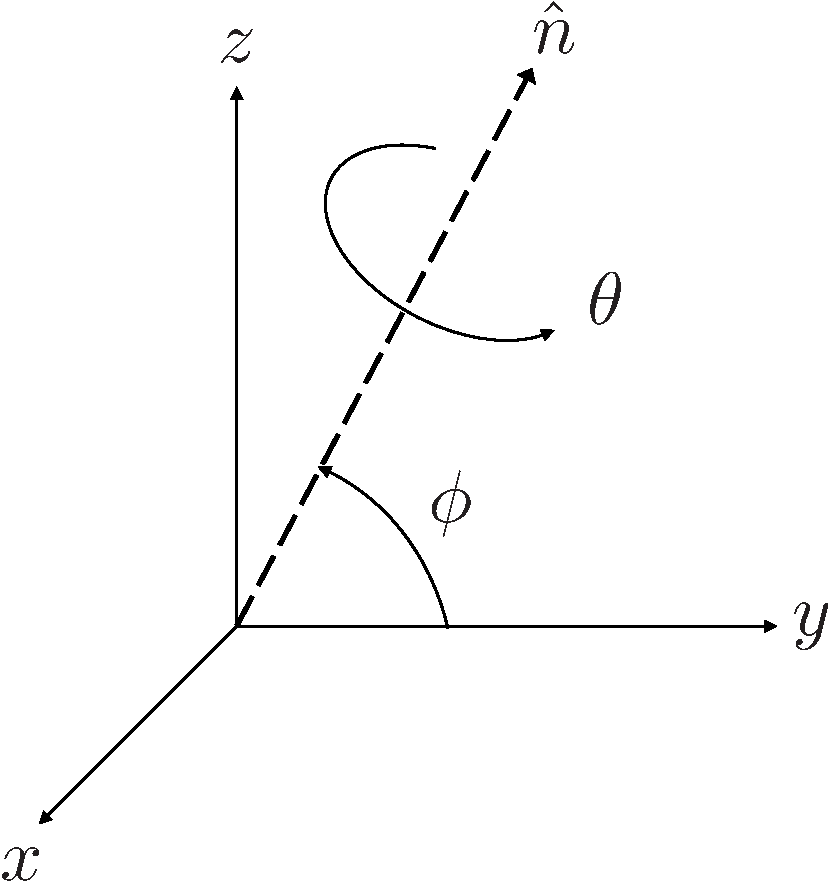
\includegraphics[width=\textwidth]{Figures/simpleRotation-crop.pdf}
\end{minipage}%
\begin{minipage}{0.65\textwidth}
\be
\hat{U}[R_{\hat{n}(\phi)}(\theta)] = 
\hat{U}[R_x( \phi)] \hat{U}[R_y( \theta)] \hat{U}[R_x(-\phi)]   
\ee
\end{minipage}\\[0.6em]%
Expanding all the $\hat{U}$'s for $\theta\to 0$ and $\phi\to 0$,
one finds:
\be
\hat{J}_z/\hbar = i [\hat{J}_y/\hbar, \hat{J}_x/\hbar]
\ee
Repeating the procedure for the $zOx$ and $xOy$,
one obtains the commutation relations $[J_y, J_z]$ and
$[J_z, J_x]$, which can be summarized by
\be
[\hat{J}_i, \hat{J}_j] = i\hbar \epsilon_{ijk}\hat{J}_k
\label{eq:g64}
\ee
%%% 06 OKAY
The algebra of the generators (Eq.~\eqref{eq:g64}) allows us to find eigenvalues
and eigenvectors of $\hat{\vec{J}}$: one can \emph{diagonalize} $\hat{\vec{J}}$.
Since $\hat{J}_i$ do not commute with each other $\rightarrow$ they
\emph{can not} be diagonalized simultaneously.

One can, however, diagonalize one of the $\hat{J}_i$
simultaneously with $\hat{\vec{J}} \cdot \hat{\vec{J}} = \hJtwo$, as the latter
is a scalar under rotation and, therefore,
commutes with any of the $\hat{J}_i$:
\be
[\hat{J}_i, \hJtwo] = 0
\ee
Let us define
\be
\hat{J}_\pm = \hat{J}_x \pm i \hat{J}_y,\quad \hat{J}_0 = \hat{J}_z
\ee
One can show (\emph{Exercise}) the following results using Eq.~\eqref{eq:g64}:
\begin{align}
[\hat{J}_0, \hat{J}_\pm] = \pm \hbar \hat{J}_\pm,\quad [\hat{J}_+,\hat{J}_-] = 2\hbar \hat{J}_0\\
\hJtwo = 1/2 (\hat{J}_+\hat{J}_- + \hat{J}_-\hat{J}_+) + \hat{J}_0^2\\
\hat{J}_\pm \hat{J}_\mp = \hJtwo - \hat{J}_0(\hat{J}_0+1)
\end{align}
With the help of these relationships, one can show that:
\begin{itemize}
\item Let $\ket{jm}$ be the simultaneous eigenvectors of $\hJtwo$ and $\hat{J}_0$.
Starting from any $\ket{jm}$, one can construct a set
%%% 07 OKAY
of $2j+1$ orthogonal vectors by repeated application
of $\hat{J}_\pm$ $\rightarrow$ these vectors span a subspace of $(2j+1)$
dimensions of $H$: $\epsilon(j)$
\item The eigenvectors $\ket{jm}$ are such that:
\be
\begin{aligned}
\hJtwo    \ket{jm} &= j(j+1)\hbar^2 \ket{jm}\\
\hat{J}_0 \ket{jm} &=   m   \hbar  \ket{jm}
\end{aligned}
\ee
with
\be
j = 0,\,1/2,\,1,\,3/2,\ldots
\ee
and
\be
m = -j, -j+1, -j+2,\ldots,j-2,j-1,j
\ee

\begin{center}
\textcolor{red}{\fbox{
\begin{tabular}{l}
If you \emph{have not} derived the above results before,\\
I urge you to take this opportunity to derive them\\
now: see Le~Bellac
\end{tabular}
}}
\end{center}

\end{itemize}

In general, one needs further quantum numbers to specify
completely the state of the system $\rightarrow$ \textit{e.g.} energy, parity,
etc. They cam be discrete or continuous; let us denote
the quantum number collectively by $\tau$, so that
\be
\ket{jm} \to \ket{\tau,jm}
\ee
with
\be
\bra{\tau^\prime,j^\prime m^\prime}\ket{\tau,jm} \equiv 
\delta_{\tau^\prime\tau} \delta_{j^\prime j} \delta_{m^\prime m}
\ee
where the $\delta_{\tau^\prime\tau}$ is Kronecker or Dirac, 
whether $\tau$ is discrete or continuous.
%%% 08 OKAY
The important properties of a standard $\ket{\tau,jm}$ basis are:
\be
\begin{gathered}
\hJtwo\ket{\tau,jm} = j(j+1)\hbar^2\ket{\tau,jm},\quad \hat{J}_0\ket{\tau,jm} = m\hbar\ket{\tau,jm}\\
\hat{J}_\pm\ket{\tau,jm} = \hbar[j(j+1)-m(m\pm 1)]^{1/2}\ket{\tau,jm\pm1}\\
\hat{J}_+\ket{\tau,j,j} = 0,\quad \hat{J}_-\ket{\tau,j,-j} = 0\\
\bra{\tau^\prime, j^\prime m^\prime}\ket{\tau, j m} = \delta_{\tau^\prime\tau}\delta_{j^\prime j}\delta_{m^\prime m},\quad
\sum_{m=-j}^{+j} \bra{\tau, jm}\ket{\tau, jm} = \mathbf{1}
\end{gathered}
\ee

Finally, using the above, one can obtain the matrix
representation $\bra{j m^\prime}\hat{J}_i\ket{j m}$.
We need a convention to construct such a matrix --
remember it is a square matrix with $(2j+1)\times(2j+1)$ components.
It is common to use the following:
\be
  \begin{BMAT}{cc}{cc}
m\setminus m^\prime
&
\begin{BMAT}(b){ccccc}{c}
 j\quad\quad	& 	j-1 	& 	\cdots 	& 	-j+1 	& 	\quad\quad-j
\end{BMAT}
\\
\begin{BMAT}(b)[4.5pt]{c}{ccccc}
j\\j-1\\\ldots\\-j+1\\-j  
\end{BMAT}
&
\left(
\begin{BMAT}(b){ccccc}{ccccc}
    (jj) 	&	(jj-1)	&	\cdots	&	\cdots	& (j-j)	 \\
    \cdots	&			&	\cdots	&			& \cdots \\ 
	\vdots	&	\vdots	&	\vdots	&	\vdots	& \vdots \\	
	\cdots	&			&	\cdots	&			& \cdots \\ 
	(-jj)	&	\cdots	&	\cdots	&	\cdots	& (-j-j) 
\end{BMAT}
\right)
 \end{BMAT}
\ee

%%% 09 OKAY

\emph{Examples:} $j=\nicefrac{1}{2}$ and $j=1$

$j=\nicefrac{1}{2}$:
\be
J_x = \frac{\hbar}{2}\begin{pmatrix}0 & 1\\1 & 0 \end{pmatrix},\quad
J_y = \frac{\hbar}{2}\begin{pmatrix}0 & -i\\i & 0\end{pmatrix},\quad
J_z = \frac{\hbar}{2}\begin{pmatrix}1 & 0\\0 & -1\end{pmatrix}
\ee
Pauli matrices: $J_i=\frac{\hbar}{2}\sigma_i$

$j=1$:
\be
J_x = \frac{\hbar}{\sqrt{2}}\begin{pmatrix}0 & 1 & 0\\1 & 0 & 1\\0 & 1 & 0  \end{pmatrix},\quad
J_y = \frac{\hbar}{\sqrt{2}}\begin{pmatrix}0 & -i & 0\\i & 0 & -i\\0 & i & 0\end{pmatrix},\quad
J_z =       \hbar           \begin{pmatrix}1 & 0 & 0\\0 & 0 & 0\\0 & 0 & -1 \end{pmatrix}
\ee

\clearpage

\subsection{Rotation matrices in Hilbert Space}
\setcounter{equation}{79}

$\rightarrow$ meaning a representation of $\hat{U}[R]$\footnote{Change of notation $(\quad)\to[\quad]$} in the basis $\ket{jm}$.

Since $\hat{U}[R]$ commutes with $\hJtwo$ and other compatible
operators (represented by $\tau$):
\be
\bra{\tau^\prime,j^\prime m^\prime} \hat{U}[R] \ket{\tau,jm} \sim \delta_{\tau^\prime \tau} \delta_{j^\prime j}
\ee
one needs to consider one $j$ at a time.

To lighten the notation, we suppress for now the index $\tau$:
\be
D^{(j)}_{m^\prime m}[R] \equiv \bra{j^\prime m^\prime} \hat{U}[R] \ket{jm}
\ee
where the $D^{(j)}_{m^\prime m}[R]$ are the \emph{Wigner matrices}.
%%% 10 OKAY
These matrices form \emph{irreducible representations} of the
rotation group.

\rule{\textwidth}{1pt}

For a group $G$ with elements $g = \{g_1,g_2,\ldots\}$, a
set of $n$-dimensional matrices $D^{(n)}(g)$ that satisfy
the group composition law:
\be
D^{(n)}(g_2)D^{(n)}(g_1) = D^{(n)}(g_2 g_1)
\ee
form an $n$-dimensional \emph{representation} of the group $G$.
If there exists a unitary transformation $U$
that \emph{does not} depend on $g$ and which for \emph{all}
$g$ reduces $D^{(n)}$ to block diagonal form,
\be
U^{-1} D^{(n)} U =
\begin{pmatrix}
D^{(n_1)} & \mathbf{0}\\
\mathbf{0} & D^{(n_2)}\\
\end{pmatrix},\quad n_1+n_2=n
\label{eq:g83}
\ee
the representation is called \emph{reducible}; if there is
no such $U$, the representation is \emph{irreducible}.

\rule{\textwidth}{1pt}

\begin{itemize}
\item Eq.~\eqref{eq:g83} implies that any transformation of $G$ can be
constructed from its irreducible representations (of known).
\item Any of the $2j+1$ vectors $\ket{jm}$ of $\epsilon(j)$ can be obtained from
an arbitrary $\ket{jm^\prime}$ by application of $D^{(j)}$, and any
matrix that commutes with all $D^{(j)}$ must be proportional
to the identity.
\end{itemize}
%%% 11 OKAY
\emph{For example}, knowing $D^{\nicefrac{1}{2}}(\theta,\phi)$, which is an irreducible
representation of the rotation group for $j=1/2$, all higher
$D^{(j)}(\theta,\phi)$ can be constructed from $D^{\nicefrac{1}{2}}(\theta,\phi)$ by using
addition of angular momentum.

\end{document}
